\documentclass[titlepage,a4paper]{article}

\usepackage{a4wide}
\usepackage[colorlinks=true,linkcolor=black,urlcolor=blue,bookmarksopen=true]{hyperref}
\usepackage{bookmark}
\usepackage{fancyhdr}
\usepackage[spanish]{babel}
\usepackage[utf8]{inputenc}
\usepackage[T1]{fontenc}
\usepackage{graphicx}
\usepackage{float}
\usepackage{amsmath}
\usepackage{multirow}
\usepackage{enumitem}
\usepackage{listings}
\usepackage{color}
\usepackage{upgreek}
 
\definecolor{codegreen}{rgb}{0,0.6,0}
\definecolor{codegray}{rgb}{0.5,0.5,0.5}
\definecolor{codepurple}{rgb}{0.58,0,0.82}
\definecolor{backcolour}{rgb}{0.95,0.95,0.92}
 
\lstdefinestyle{mystyle}{
    backgroundcolor=\color{backcolour},   
    commentstyle=\color{codegreen},
    keywordstyle=\color{magenta},
    numberstyle=\tiny\color{codegray},
    stringstyle=\color{codepurple},
    basicstyle=\footnotesize,
    breakatwhitespace=false,         
    breaklines=true,                 
    captionpos=b,                    
    keepspaces=true,                 
    numbers=left,                    
    numbersep=5pt,                  
    showspaces=false,                
    showstringspaces=false,
    showtabs=false,                  
    tabsize=2
}
 
\lstset{style=mystyle}
\lstset{language=Octave}

\pagestyle{fancy}
\fancyhf{}
\fancyhead[L]{TP2 - Grupo 5}
\fancyhead[R]{Análisis Numérico I - FIUBA}
\renewcommand{\headrulewidth}{0.4pt}
\fancyfoot[C]{\thepage}
\renewcommand{\footrulewidth}{0.4pt}


\begin{document}


\begin{titlepage}
	\hfill
\includegraphics[width=6cm]{logofiuba.jpg}
    	\centering
    	\vfill
	\huge \textbf{Análisis Numérico I\\}
	\huge \textbf{[75.12/95.04]\\}
	\huge \textbf{Curso 3\\}
	\huge \textbf{Trabajo Práctico 2}\\
	\huge \textbf{Problema de los Tres Cuerpos Restringido}
	\vskip2cm
	\large
	Grupo 5 \\
    	Primer cuatrimestre de 2019 
	\vfill

	\begin{tabular}{ |l|l|l| }
		\hline
		\multicolumn{3} { |c| } {\textbf{Integrantes del grupo}} \\ \hline
		Santa María Tomás & 92797 & tomasisantamaria@gmail.com\\ \hline
	 	Hemmingsen Lucas & 76187 & lhemmingsen@fi.uba.ar\\ \hline
	 	Huenul Matías & 102135 & matias.huenul.07@gmail.com\\ \hline
	\end{tabular}
	\vfill
    	\vfill
\end{titlepage}

\tableofcontents %Esta línea genera un indice a partir de las secciones y subsecciones creadas en el documento
	\newpage

	
\section{Introducción}\label{sec:introd}
	El objetivo del presente trabajo práctico es utilizar los distintos metodos numéricos de problema de valor inicial 
	para ecuaciones diferenciales ordinarias, para resolver el ``Problema de los Tres Cuerpos Restringido o de Euler'' 
	y realizar una comparación de los resultados con cada método.

	Los métodos que utilizaremos son el método de Euler, Runge-Kutta de orden 2 y 4, Nystr\"om y Newmark.

	


\section{Conceptos teóricos}\label{sec:conceptos}
	\subsection{Método de Euler}
	Sea $ y'(t) = f(t, y) $ una ecuación diferencial ordinaria de primer orden con condición inicial $ y(t_{0}) = y_{0} $. Se quiere obtener la solución en $ N + 1 $ puntos en un intervalo dado, uniformemente espaciado con paso $h$. 
	Se puede aproximar y(t) por su Polinomio de Taylor de primer orden:
	\begin{equation}
		y(t_{k} + h) \cong y(t_{k}) + hy'(t_{k})
	\end{equation}
	Pero como $y'(t_{k}) = f(t_{k}, y(t_{k}))$ y además $ t_{k+1} = t_{k} + h $ para todo $ 0 \leq k \leq N $, esta expresión se puede reescribir como:
	\begin{equation}
		y(t_{k+1}) \cong t(t_{k}) + hf(t_{k}, y(t_{k}))
	\end{equation}
	Este método puede usarse para resolver sistemas de ecuaciones diferenciales,  aplicando lo anterior a cada componente del sistema.\\
	El error cometido con este método se debe en parte al error de truncamiento local (dado por el Teorema de Taylor) en cada paso $k$ y al error cometido por utilizar como condición inicial en dicho paso $ y_{k-1} $, obtenido en el anterior. Se puede demostrar que si el problema está bien planteado, el error total es $ e = O(h) $.
	\subsection{Método de Runge-Kutta}
	Los métodos de Runge-Kutta son una familia de métodos para resolver numéricamente ecuaciones diferenciales ordinarias de orden $ n $, de la forma $ y'(t) = f(t, y) $, con condición inicial $ y(t_{0}) = y_{0} $.
	En particular para este Trabajo Práctico se desea hallar soluciones utilizando los métodos de orden 2 y orden 4, cuyas expresiones se mencionan a continuación.
	\subsubsection{Euler Modificado}
	Dado el Problema de Valor Inicial, se puede expresar la solución de la ecuación diferencial ordinaria de orden 2 de la siguiente forma:
	\begin{equation}
		y_{n+1} = y_n + \frac{h}{2} (k_1 + k_2)
	\end{equation}
	donde $ k_1, k_2 $ son:

	\begin{align*}
		k_1 &= f(t_i, y_i)\\
		k_2 &= f(t_i + h, y_i + hk_1)
	\end{align*}

	subsubsection{Runge-Kutta de orden 4}

	\begin{equation}
		y_{n+1} = y_n + \frac{h}{6} (k_1 + 2k_2 + 2k_3 + k_4)
	\end{equation}
	donde $ k_1, k_2, k_3, k_4 $ son:

	\begin{align*}
		k_1 &= f(t_i, y_i) \\
		k_2 &= f(t_i + \frac{h}{2}, y_i + h \frac{k_1}{2})\\
		k_3 &= f(t_i + \frac{h}{2}, y_i + h \frac{k_2}{2})\\
		k_4 &= f(t_i + h, y_i + h k_3)
	\end{align*}

	El error global cometido por estos métodos es $ e = O(h^n) $.
 
	\subsection{Método de Nystr\"om}

	El método de Nystr\"om es un método de paso múltiple, que aplica de la siguiente manera, dada una EDO de primer orden:

	\begin{align*}
		y'(t) &= f(t, y)\\
		y(t_{0}) &= y_{0}
	\end{align*}

	Las ecuaciones adoptan la siguiente forma: 

	\begin{align*}
		y_{i+1} = y_{i-1} + 2h y'(t_i), i = 1, 2,..., n - 1
	\end{align*}

	Se observa que se debe obtener un valor de arranque, $ y_1 $, para poder comenzar a resolver el problema. En el presente trabajo práctico se utilizará el método de Euler Modificado para aproximar el valor necesario. 

	\subsection{Método de Newmark}
	Este método se obtiene a partir de la serie de Taylor y es usado para resolver EDOs de segundo orden.
	Sea $ y'' = f(t, y, y') $, entonces las ecuaciones son:
	\begin{equation}
		\begin{cases}
		y(t_{k+1}) = y(t_{k}) + hy'(t_{k}) + \frac{h^2}{2}[\alpha f(t_{k}; y(t_{k});y'(t_{k})) + (1 - \alpha) f(t_{k+1}, y(t_{k+1}); y'(t_{k+1}))]\\
		y'(t_{k+1}) = y'(t_{k}) + h[\beta f(t_{k}; y(t_{k}); y'(t_{k}) + (1-\beta)f(t_{k+1},;y(t_{k+1});y'(t_{k+1}))]
		\end{cases}
	\end{equation}

	\subsection{Sistema de ecuaciones diferenciales de primer orden}\cite{burden_system_diff_eq}
		Sea un sistema de ecuaciones diferenciales de primer orden con la forma:

		\begin{equation}
			\label{eq1}
			\begin{cases}
				\frac{du_{1}}{dt}=f_{1}(t,u_{1},u_{2},...,u_{m})\\
				\frac{du_{2}}{dt}=f_{2}(t,u_{1},u_{2},...,u_{m})\\
				\vdots\\
				\frac{du_{m}}{dt}=f_{m}(t,u_{1},u_{2},...,u_{m})
			\end{cases}
		\end{equation}

		para $a \leq t \leq b$, con condiciones iniciales:
		\begin{equation}
			\label{eq2}
			u_{1}(a) = \alpha_{1}, u_{2}(a)=\alpha_{2}, \dots, u_{m}(a)=\alpha_{m}
		\end{equation}
		El objetivo es encontrar \emph{m} funciones $u_{1}(t),u_{2}(t),\dots,u_{m}(t)$ que satisfacen 
		cada una de las ecuaciones diferenciales junto con las condiciones iniciales.
		Los métodos para resolver sistemas de ecuaciones diferenciales de primer orden son simplemente 
		generalizaciones de los métodos para una sola ecuación diferencial presentados anteriormente.

	\subsection{Ecuaciones diferenciales de orden mayor a 1}\cite{burden_higher_order_diff_eq}
			Una ecuación diferencial de grado \emph{m}
			\begin{equation}
				y^{(m)}(t)=f(t,y,y',\dots,y^{(m-1)})
			\end{equation}
			con $a \leq t \leq b$ y condiciones iniciales $y(a)=\alpha_{1},y'(a)=\alpha_{2},\dots,y^{(m-1)(a)=\alpha_{m}}$ 
			puede convertirse a un sistema de ecuaciones de la forma de \eqref{eq1} y \eqref{eq2}.

			Sea $u_{1}(t)=y(t),u_{2}(t)=y'(t),\dots,u_{m}(t)=y^{(m-1)}(t)$. Esto produce el sistema de ecuaciones diferenciales 
			de primer orden

			\begin{equation}
				\frac{du_{1}}{dt}=\frac{dy}{dt}=u_{2},\frac{du_{2}}{dt}=\frac{dy'}{dt}=u_{3},\dots,\frac{du_{m-1}}{dt}=\frac{dy^{(m-2)}}{dt}=u_{m}
			\end{equation}

			y

			\begin{equation}
				\frac{du_{m}}{dt}=\frac{dy^{(m-1)}}{dt}=y^{(m)}=f(t,y,y',\dots,y^{(m-1)})=f(t,u_{1},u_{2},\dots,u_{m})
			\end{equation}

			con condiciones iniciales

			\begin{equation}
				u_{1}(a)=y(a)=\alpha_{1}, u_{2}(a)=y'(a)=\alpha_{2},\dots,u_{m}(a)=y^{(m-1)}(a)=\alpha_{m}
			\end{equation}
\section{Desarrollo}\label{sec:desarrollo}
	\subsection{Parte A}\label{sec:parteA}

		Tenemos el siguiente sistema de ecuaciones diferenciales de segundo orden que representan el movimiento de un satélite
		viajando entre la tierra y la luna e influenciado gravitatoriamente solo por estos dos cuerpos:
		\begin{equation}
			\begin{cases}
				x''_{1} = 2x'_{2} + x_{1} - \eta\frac{x_{1} + \mu}{d_{1}^{3}} - \mu\frac{x_{1}-\eta}{d_{2}^{3}}\\
				x''_{2} = -2x'_{1} + x_{2} - \eta\frac{x_{2}}{d_{1}^{3}} - \mu\frac{x_{2}}{d_{2}^{3}}
			\end{cases}
		\end{equation}

		Siendo $d_{1}=\sqrt{(x_{1}+\mu)^{2} + x_{2}^{2}}$ y $d_{2}=\sqrt{(x_{1}-\eta)^{2} + x_{2}^{2}}$.

		Sea:

		\begin{equation}
			\begin{cases}
				v_{1}(t) = x'_{1}(t)\\
				v_{2}(t) = x'_{2}(t)
			\end{cases}
		\end{equation}

		Entonces podemos transformar el sistema de ecuaciones anterior en un sistema de cuatro ecuaciones 
		diferenciales de primer orden:

		\begin{equation}
			\begin{cases}
				x'_{1}(t) = v_{1}(t)\\
				v'_{1}(t) = 2v_{2}(t) + x_{1}(t) - \eta\frac{x_{1}(t) + \mu}{d_{1}(t)^{3}} - \mu\frac{x_{1}(t) - \eta}{d_{2}(t)^{3}}\\
				x'_{2}(t) = v_{2}(t)\\				
				v'_{2}(t) = -2v_{1}(t) + x_{2}(t) - \eta\frac{x_{2}(t)}{d_{1}(t)^{3}} - \mu\frac{x_{2}(t)}{d_{2}(t)^{3}}
			\end{cases}
		\end{equation}

		Con valores iniciales en $t=t_{0}$:

		\begin{equation}
			\begin{cases}
				x_{1}(t_{0}) = x_{1_{0}}\\
				v_{1}(t_{0}) = v_{1_{0}}\\
				x_{2}(t_{0}) = x_{2_{0}}\\				
				v_{2}(t_{0}) = v_{2_{0}}\\
			\end{cases}
		\end{equation}

	\subsection{Parte B}\label{sec:parteB}
		Ahora resolvamos el problema numéricamente con la función \emph{lsode} de \emph{Octave}.		
		Primero creamos la función \emph{yprima}, que representa a la función \emph{f(t,y)}.
		A continuación se detalla el código de la misma:

		\lstinputlisting[language=Octave]{yprima.m}

		Luego, desde la consola de \emph{Octave} ejecutamos la función \emph{lsode} con la función 
		\emph{yprima} como entrada, con una posición inicial $(x_{1}, x_{2}) = (1.2, 0)$ y velocidad inicial 
		$(v_{1}, v_{2}) = (0, -0.8)$ en el intervalo $[t_{0}, t_{1}) = [0, 2]$ con un $h=0.01$.
		Para ello, ejecutamos:

			\begin{lstlisting}
				[y]=lsode('yprima',[1.2 0 0 -0.8],0:0.01:2)			
			\end{lstlisting}
		con lo que en la última iteración (en t=2) obtenemos una posición final 
		$(x_{1}, x_{2}) = (-0.51306, 0.07881)$ y una velocidad final $(v_{1}, v_{2}) = (-1.18383, -0.48564)$.

		A continuación se muestra un gráfico de la trayectoria del satélite, que se mueve desde el extremo
		derecho del gráfico hacia la izquierda.
		\begin{figure}[H]
			\centering
			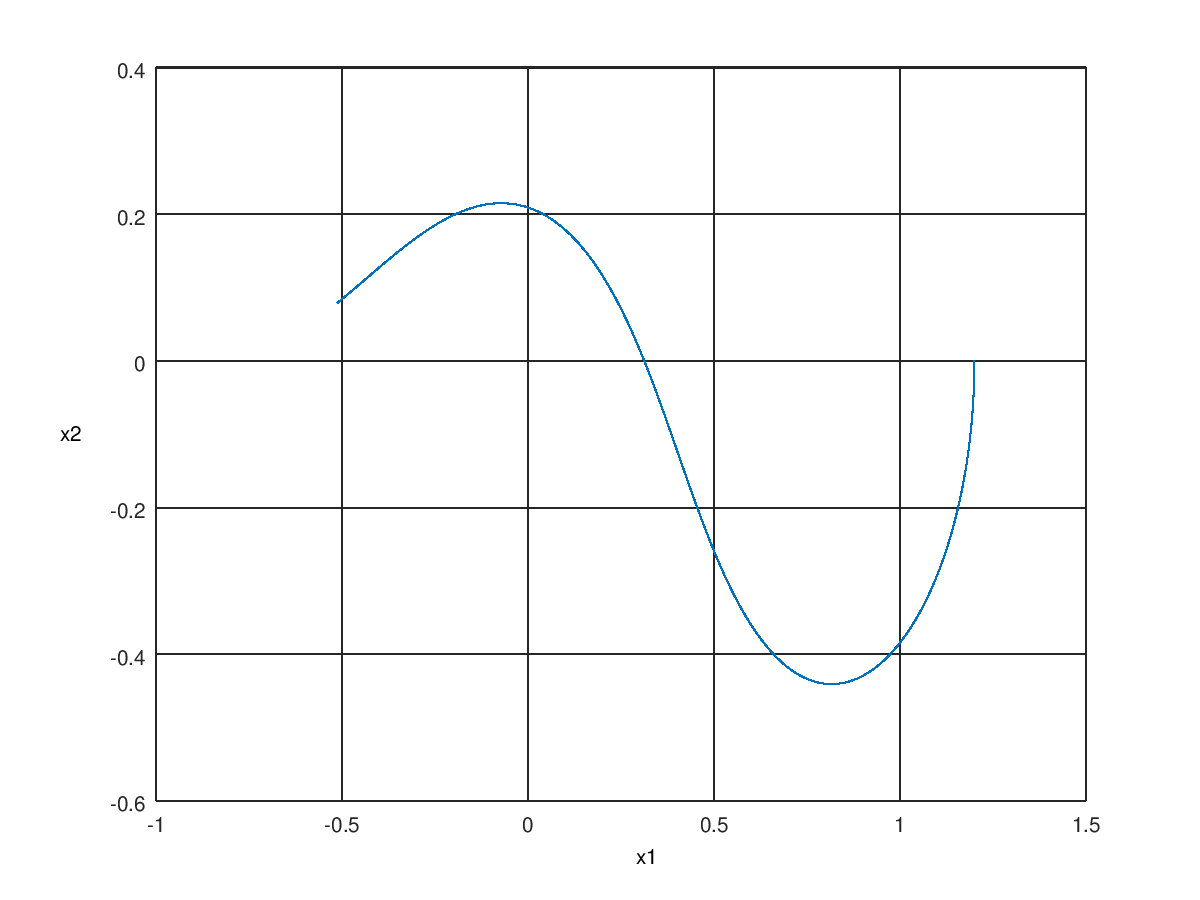
\includegraphics[width=0.9\textwidth]{parteb.png}
			\caption{\label{fig:parteb}Trayectoria del satélite obtenida con \emph{lsode}.}
		\end{figure}

	\subsection{Parte C}\label{sec:parteC}
	Veremos ahora como se modifica la trayectoria aumentando el paso $h$. Para ello implementamos siguiente función.\\

	\lstinputlisting[language=Octave]{lsode_con_distintos_h.m}

	En el siguiente gráfico se puede observar lo obtenido para cuatro valores  de $h$ en particular, utilizando como condiciones iniciales las mismas que al comienzo de la parte b.\\
	\begin{figure}[H]
		\centering
		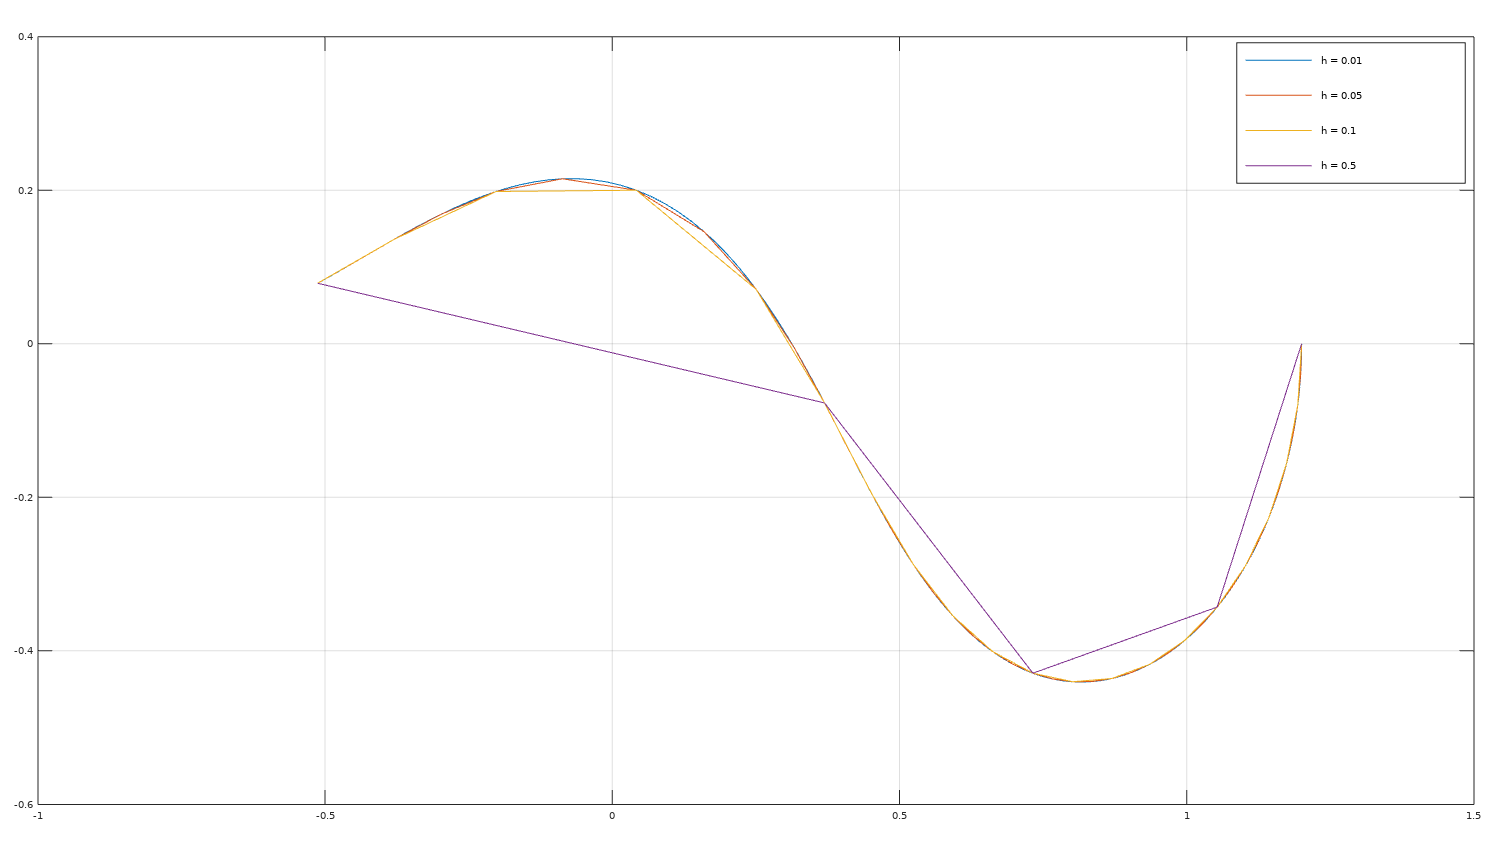
\includegraphics[width=0.9\textwidth]{partec.png}
		\caption{\label{fig:partec}Trayectoria obtenida con distintos valores de \emph{h}.}
	\end{figure}

	\subsection{Parte D}\label{sec:parteD}
	Resolveremos ahora el sistema en el intervalo $[0; 2]$ mediante el método de Euler. Las ecuaciones son:
	\begin{equation}
		\label{inicial}
		\begin{cases}
			x_1 (t_{k+1}) = x_1 (t_{k}) + hv_1 (t_{k})\\
			v_1 (t_{k+1}) = x_2 (t_{k}) + h(2v_2 (t_{k}) + x_1 (t_{k}) - \eta\frac{x_1 (t_{k}) - \mu}{d_1 (t_{k})^{3}})\\
			x_2 (t_{k+1}) = x_2 (t_{k}) + hv_2 (t_{k})\\
			v_2 (t_{k+1}) = v_2 (t_{k}) + h(-2v_1 (t_{k}) + x_2 (t_{k}) - \eta\frac{x_2 (t_{k})}{d_1 (t_{k})^{3}}) - \mu\frac{x_2 (t_{k})}{d_2 (t_{k})^{3}})\\
		\end{cases}
	\end{equation}

	El código de la función implementada en \emph{Octave} para la resolución con este método se muestra a continuación.
	\lstinputlisting[language=Octave]{euler.m}
	Primero utilizamos como condición inicial el vector $ y_0 = (1,2; 0; 0; -0,8) $ y como tolerancia el valor $ h = 0.01 $.\\
	Los resultados para cada $t$ del intervalo se encuentran en el archivo \emph{resultados-parte-d.txt}.\\
	En particular, el resultado obtenido para $t=2$ es:
	\begin{equation}
		y(2) = (-0.54958; -1.49872; 0.21286; -0.03654)
	\end{equation}
	La trayectoria obtenida en este caso es la siguiente.\\
	\begin{figure}[H]
		\centering
		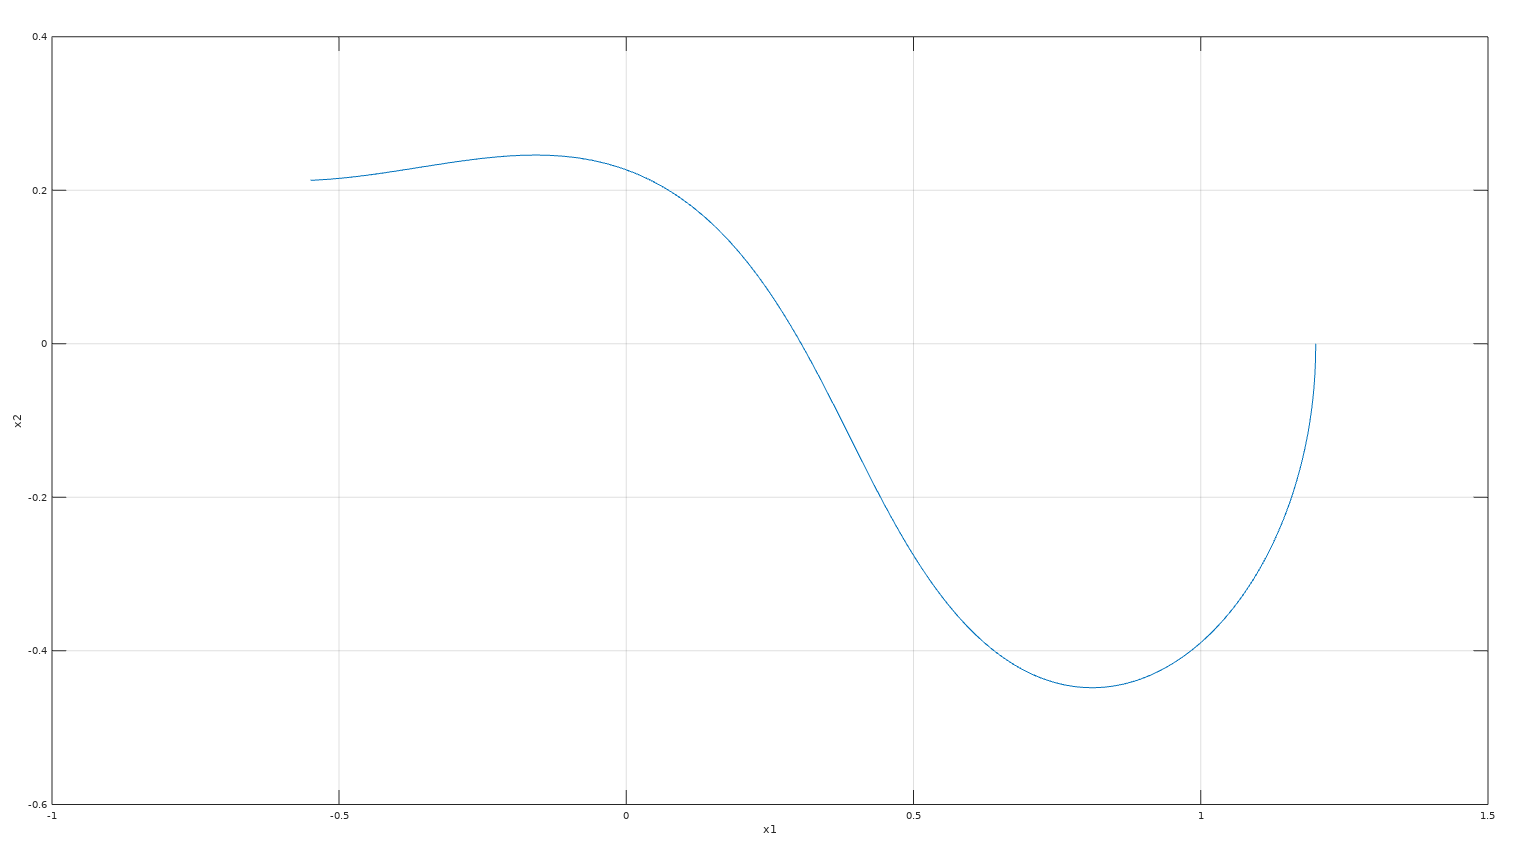
\includegraphics[width=0.9\textwidth]{parted.png}
		\caption{\label{fig:parted}Trayectoria del satélite obtenida con el método de Euler.}
	\end{figure}
	Calcularemos ahora el error cometido por este método. Asumiendo como valor correcto el obtenido por la función \emph{lsode} en la parte B, el error es:
	\begin{equation}
		e = (x_{1_{lsode}}; x_{2_{lsode}}) - (x_{1_{euler}}; x_{2_{euler}}) = (0,036514; -0,134042)
	\end{equation}
	Modificando el paso \emph{h}, vemos que el error es proporcional a éste, de acuerdo a la teoría. Por ejemplo, para $ h = 0.001 $ el error es $ e = (0.0063200;-0.0160951) $ y para $ h = 0.1 $ es $ e = (0,0098268;0.61340) $. \\
	En el siguiente gráfico se puede ver que la dependencia entre h y la norma del error absoluto es aproximadamente lineal.\\
	\begin{figure}[H]
		\centering
		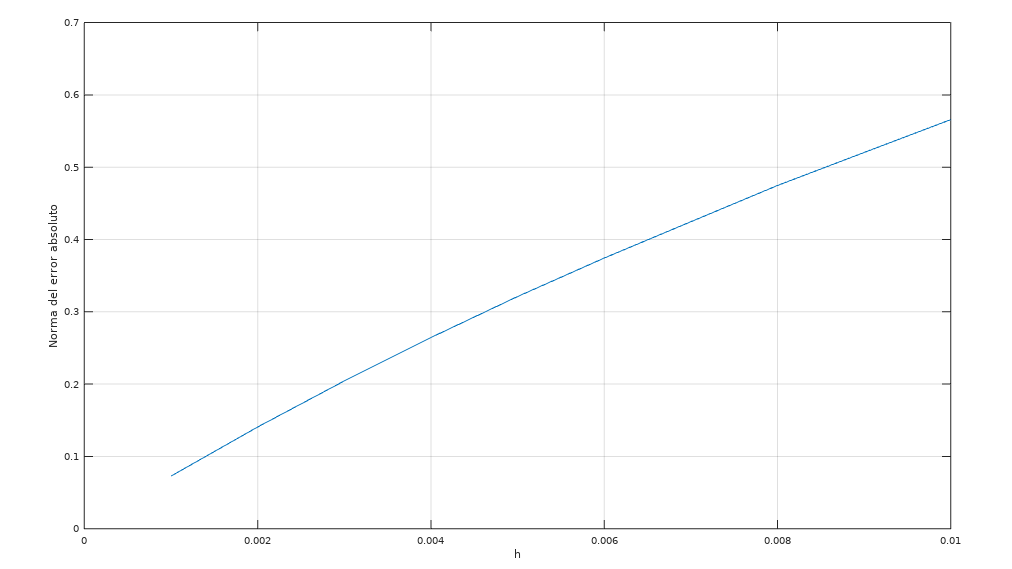
\includegraphics[width=0.9\textwidth]{error_euler.png}
		\caption{\label{fig:error_euler}Error cometido con el método de Euler en función de \emph{h}.}
	\end{figure}
	

	\subsection{Parte E}\label{sec:parteE}
	Resolveremos el sistema en el intervalo $[0; 2]$ mediante el método de Euler Modificado (RK2) y Runge-Kutta de orden 4, utilizando las mismas ecuaciones planteadas en \ref{inicial}. Los método de Runge-Kutta consiguen órdenes de convergencia similares a los de Taylor, pero no necesitan obtener las derivadas de la función $ f(t, y) $.
	El código de la función implementada en \emph{Octave} para la resolución con Euler Modificado se muestra a continuación.
	\lstinputlisting[language=Octave]{modified_euler.m}

	Como mismas condiciones iniciales planteadas en la parte B del presente Trabajo Práctico. Se analizaron también los resultados tomando intervalos $ h = 0.1 $ y $ h = 0.001 $. Los resultados de cada corrida se encuentran en el repositorio en los siguientes archivos: \emph{modified\_euler-0.01.txt}, \emph{modified\_euler-0.1.txt} y \emph{modified\_euler-0.001.txt}.\\ 
	El resultado obtenido para $ t = 2 $, con $ h = 0.01 $ es:
	\begin{equation}
		y(2) = (-0.513149; -1.189898; 0.084632; -0.468974)
	\end{equation}
	\begin{figure}[H]
		\centering
		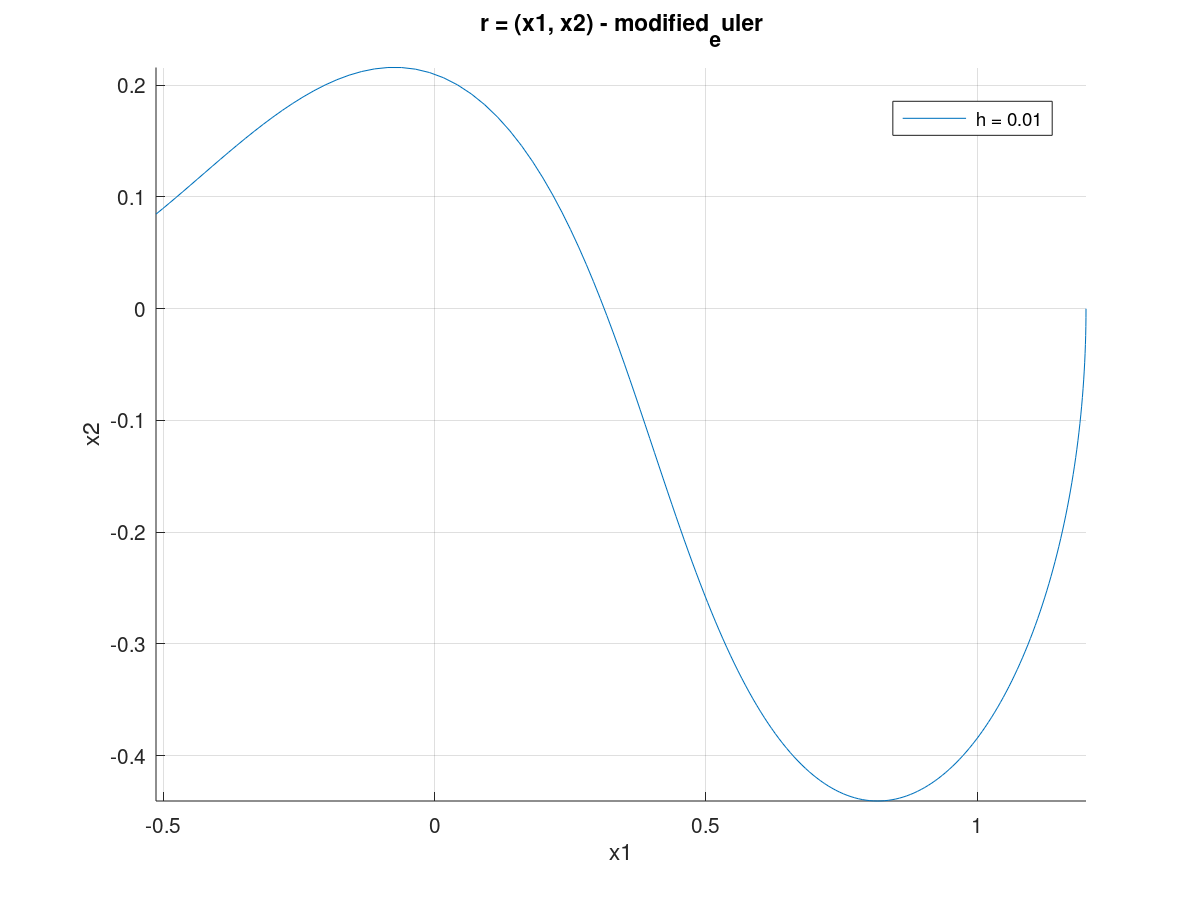
\includegraphics[width=0.9\textwidth]{modified_euler.png}
		\caption{\label{fig:parted}Trayectoria del satélite obtenida con el método de Euler Modificado.}
	\end{figure}
	Se comprueba que, como dice la teoría, modificando el intervalo $ h $ se tiene más precisión en los resultados, ya que para $ h = 0.001 $,
	\begin{align*}
		y(2) &= (-0.513058; -1.183882; 0.078874; -0.485479)\\
		x(2) &= (-0.513058; 0.078874)\\
		v(2) &= (-1.183882; -0.485479)
	\end{align*}
	cuyos resultados se aproximan al vector determinado por la función \emph{lsode} de Octave.\\

	Para la resolución mediante el método de Runge-Kutta de orden 4 se implementó la siguiente funcion:
	\lstinputlisting[language=Octave]{rk4.m}

	Con las mismas condiciones iniciales, y analizando en los mismos intervalos de $ h $ que en la resolución para el 2do orden, se llegaron a los siguientes resultados:
	\begin{align*}
		y(2) &= (-0.496993; -1.107211; 0.073956; -0.541870), h = 0.1\\
		y(2) &= (-0.513059; -1.183832; 0.078815; -0.485642), h = 0.01\\
		y(2) &= (-0.513060; -1.183835; 0.078817; -0.485633), h = 0.001
	\end{align*}

	Los resultados de cada corrida se encuentran en el repositorio en los siguientes archivos: \emph{rk4-0.01.txt}, \emph{rk4-0.1.txt} y \emph{rk4-0.001.txt}. La trayectoria obtenida es la siguiente:
	
	\begin{figure}[H]
		\centering
		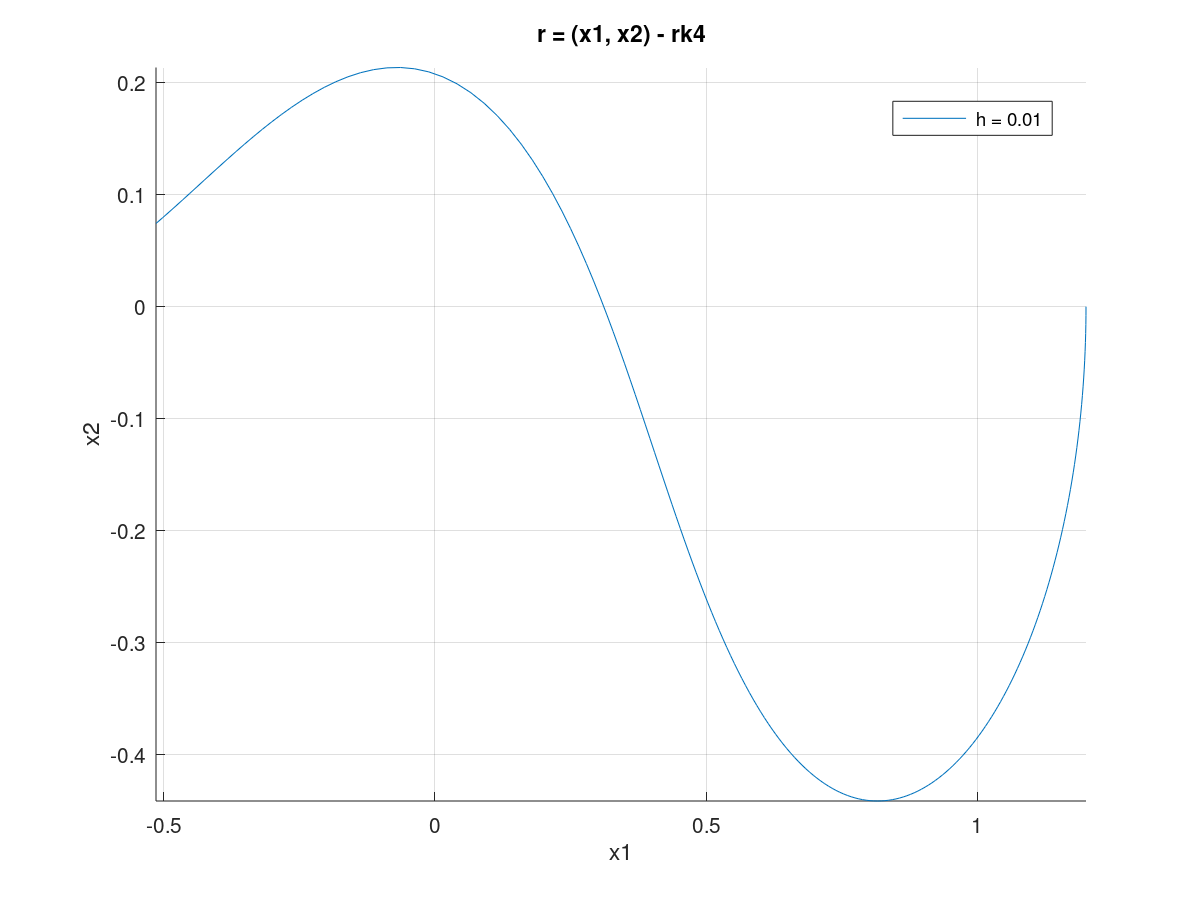
\includegraphics[width=0.9\textwidth]{rk4.png}
		\caption{\label{fig:parted}Trayectoria del satélite obtenida con el método de Runge-Kutta orden 4.}
	\end{figure}

	Para calcular el error absoluto, se implementó la siguiente función que recibe por parámetro el método sobre el cual calcularlo:
	\lstinputlisting[language=Octave]{error_segun_metodo.m}

	Al llamarlo mediante las siguientes expresiones:

	\begin{lstlisting}
		>> error_segun_metodo('modified_euler', 'yprima', 0, 2, 0.01, [1.2 0 0 -0.8])
		(e_x1, e_x2) = (0.00008750, -0.00581758)

		>> error_segun_metodo('rk4', 'yprima', 0, 2, 0.01, [1.2 0 0 -0.8])
		(e_x1, e_x2) = (-0.00000185, -0.00000042)
	\end{lstlisting}

	Se puede observar que, al igual que en el método de Euler, al hacer más pequeño el paso $ h $ el error tiende a ser más pequeño. Además, se observa que el método de Runge-Kutta de orden 4 converge más rápido que los otros métodos.

	\begin{lstlisting}
		>> error_segun_metodo('modified_euler', 'yprima', 0, 2, 0.001, [1.2 0 0 -0.8])
		(e_x1, e_x2) = (-0.00000351, -0.00005982)

		>> error_segun_metodo('rk4', 'yprima', 0, 2, 0.001, [1.2 0 0 -0.8])
		(e_x1, e_x2) = (-0.00000137, -0.00000293)
	\end{lstlisting}

	\subsection{Parte F}\label{sec:parteF}
	Utilizando las mismas condiciones iniciales ya planteadas, procederemos a resolver el sistema mediante el método de Nystrom, utilizando como método de arranque para obtener $ y_1 $ a Euler Modificado. El código que implementa la función está preparado para correr utilizando cualquier método de los ya presentados pasando como parámetro el archivo .m que lo contiene:
	\begin{lstlisting}
		[Y] = nystrom('yprima', 0, 2, 0.01, [1.2 0 0 -0.8], 'modified_euler')
	\end{lstlisting}

	\lstinputlisting[language=Octave]{nystrom.m}

	Los resultados de cada corrida se encuentran en el repositorio en los siguientes archivos: \emph{nystrom-0.01.txt}, \emph{nystrom-0.1.txt} y \emph{nystrom-0.001.txt}. Con las mismas condiciones iniciales, y analizando en los mismos intervalos de $ h $ que en las resoluciones anteriores, se llegaron a los siguientes resultados:
	\begin{align*}
		y(2) &= (-0.499271; -0.669870; 0.548925; -0.066994), h = 0.1\\
		y(2) &= (-0.512801; -1.187857; 0.084554; -0.470498), h = 0.01\\
		y(2) &= (-0.513058; -1.183877; 0.078875; -0.485480), h = 0.001
	\end{align*}

	Mientras que la trayectoria del satélite se puede observar en el siguiente gráfico:

	\begin{figure}[H]
		\centering
		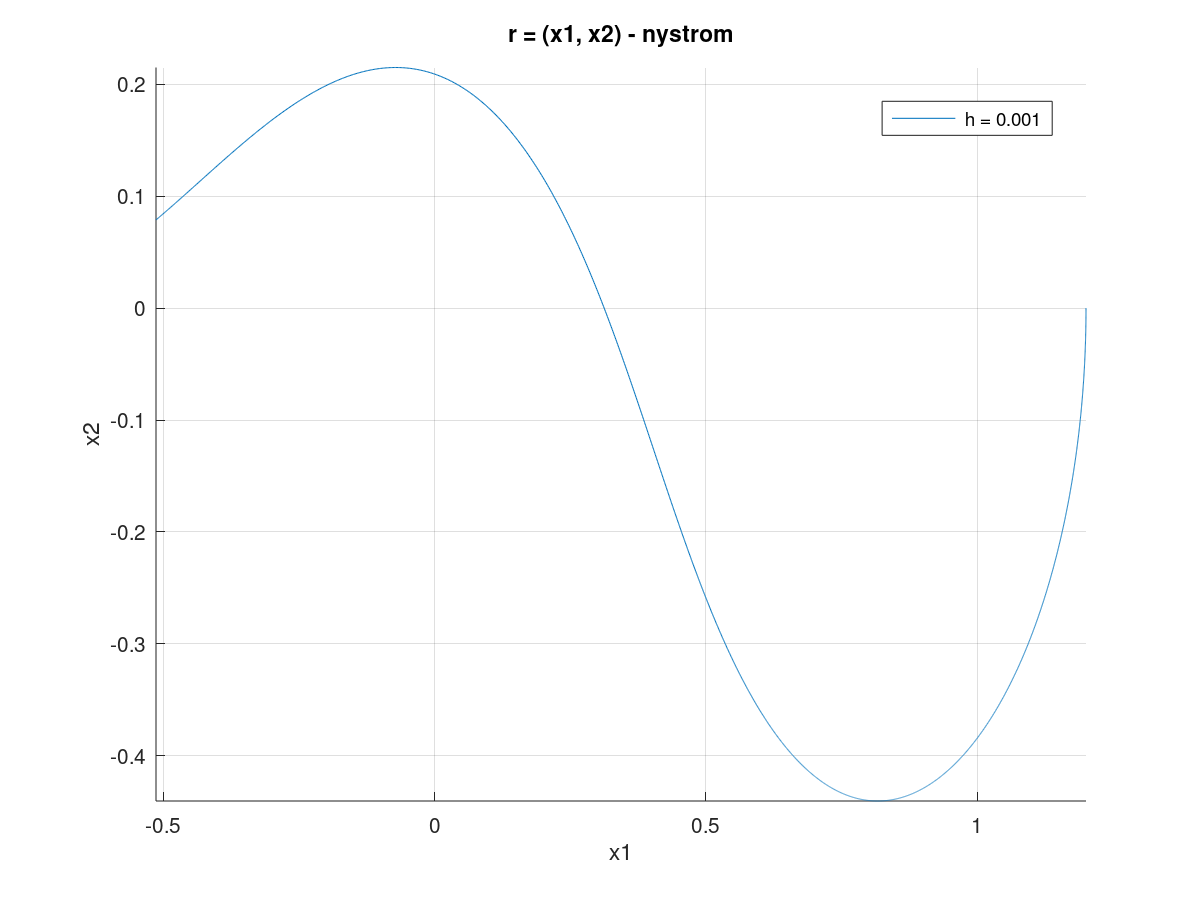
\includegraphics[width=0.9\textwidth]{nystrom.png}
		\caption{\label{fig:parted}Trayectoria del satélite obtenida con el método de Nystrom.}
	\end{figure}

	Para calcular el error absoluto, se implementó la siguiente función que recibe por parámetro el método sobre el cual calcularlo:
	\lstinputlisting[language=Octave]{error_segun_metodo_arranque.m}

	Al llamarlo mediante las siguientes expresiones:

	\begin{lstlisting}
		>> error_segun_metodo_arranque('nystrom', 'yprima', 0, 2, 0.1, [1.2 0 0 -0.8], 'modified_euler')
		(e_x1, e_x2) = (-0.01378996, -0.47011101)
		>> error_segun_metodo_arranque('nystrom', 'yprima', 0, 2, 0.01, [1.2 0 0 -0.8], 'modified_euler')
		(e_x1, e_x2) = (-0.00025996, -0.00573996)
		>> error_segun_metodo_arranque('nystrom', 'yprima', 0, 2, 0.001, [1.2 0 0 -0.8], 'modified_euler')
		(e_x1, e_x2) = (-0.00000375, -0.00006071)
	\end{lstlisting}

	se observa que nuevamente al modificar el intervalo de $ h $, se realizan más iteraciones y en consecuencia el error absoluto es más pequeño.

	%\subsection{Parte G}\label{sec:parteG}

\begin{thebibliography}{9} 
	\bibitem{burden_system_diff_eq} 
		Richard L. Burden, J. Douglas Faires\\
		\textit{Numerical Analysis (9th edition)}. \\
		Brooks/Cole - Cengage Learning\\
		Sección 5.9 Higher Order Equations and Systems of Differential Equations\\
		Páginas 328-334

	\bibitem{burden_higher_order_diff_eq} 
		Richard L. Burden, J. Douglas Faires\\
		\textit{Numerical Analysis (9th edition)}.\\ 
		Brooks/Cole - Cengage Learning\\
		Sección 5.9 Higher Order Equations and Systems of Differential Equations\\
		Páginas 334-336
	\bibitem{burden_euler}
		Richard L. Burden, J. Douglas Faires\\
		\textit{Numerical Analysis (9th edition)}. \\
		Brooks/Cole - Cengage Learning\\
		Sección 5.2 Euler's Method\\
		Páginas 266-268
	\bibitem{error_analysis_euler_method}
		UBC Math - University of British Columbia\\
		Error Analysis of the Euler Method\\
		\url{http://www.math.ubc.ca/~israel/m215/euler2/euler2.html}
	 
\end{thebibliography}



\end{document}